\section{Experiments}\label{sect:exp}

This section presents our experimental evaluation. In the first part
(Section~\ref{sect:exp-mitig}), we show the benefits coming from the
introduction of sandboxing in cloud applications. In detail, we
reproduce a sample of CVEs affecting open source software, and
showcase how the sandbox mitigates the exploits. In the second part
(Section~\ref{sect:exp-perf}), we analyze the performance
overhead. Specifically, we implement an application that performs
various operations on media resources, and then evaluate the
degradation of latency when sandboxing and eBPF-based monitoring are
activated. The tests have been executed on a workstation with Arch
Linux, kernel version 6.4, an AMD Ryzen 5 7600X CPU, 32 GB RAM, and 1
TB SSD.

\subsection{Mitigation of vulnerabilities}\label{sect:exp-mitig}

To demonstrate the importance of the introduction of sandboxing, we
selected the sample of high severity vulnerabilities reported in
Table~\ref{table:cve}. These vulnerabilities affect software
extensively used in cloud application development such as FFmpeg,
ImageMagick, OpenSSL and Exiftool. For each of them, we installed on
the system a vulnerable version of the program or library, and then
verified it was exploitable using public Proof of Concepts when the
input is sent through programmatic APIs or web
interfaces. Subsequently, we leveraged \dmng to generate least
privilege policies as explained in
Section~\ref{sect:cloud-instrum}. Finally, we repeated the execution
of the previous tests starting each vulnerable component with our
sandboxer. When benign input was submitted to the application, we were
successfully able to conduct the tests without loss of
functionality. When instead malicious input was used, Landlock
correctly blocked the exploit, limiting access to only resources
listed in the policy. We highlight that, in general, similar
protections extend to a broader set of CVEs.


\begin{table}[!t]
  \footnotesize
  \caption{\label{table:cve} Sample of CVEs reproduced in our evaluation}
  \setlength{\tabcolsep}{0.2cm}
  \begin{tabularx}{\columnwidth}{ l l l >{\raggedright\arraybackslash}X}
    \toprule
    {\bf CVE} & {\bf Software} & {\bf Version} & {\bf Description}\\
    \toprule
    CVE-2016-1897  & \multirow{2}{*}{FFmpeg} & \multirow{2}{*}{v2.x} & A crafted AVI video is used to read arbitrary \\
    CVE-2016-1898  & & & files \\
    \midrule
    CVE-2020-29599  & ImageMagick  & v7.0.10-36  & A bug in the PDF codec enables arbitrary code execution \\
    \midrule
    CVE-2022-1292  & OpenSSL  & v3.0.2 & Improper sanitisation allows command injection \\
    \midrule
    CVE-2021-22204   & ExifTool        &  v12.23 & Improper neutralization of user data in the DjVu file format is used to run arbitrary executables \\
    \bottomrule
  \end{tabularx}
\end{table}

\subsection{Overhead}\label{sect:exp-perf}

As mentioned in Section~\ref{sect:motivation}, an important use case
for cloud applications is represented by services that handle media
resources such as videos, photos and audio. Therefore, to evaluate the
overhead associated with our approach we implemented a Rust
application that, upon receiving a request, leverages third-party
software to apply several transformations on a media resource. Our
goal is to measure the latency, or rather the time taken by the
application to perform a given operation. Three test configurations
are used: 1)~no sandboxing is applied, hence no protection,
2)~sandboxing is enabled leveraging our Landlock-based sandboxer, and
3)~sandboxing is enabled plus eBPF-based continuous monitoring
provided by \dmng is activated. Each operation is repeated 1000 times,
and the measures are reported with 95\% confidence intervals. Moreover, we focus on the
server-side execution time, hence we do not consider the delay
introduced by the network, which may make harder to visualize latency
degradation for short-lived operations.

\begin{figure*}[t!]
  \begin{subfigure}[b]{0.5\linewidth}
    \centering
    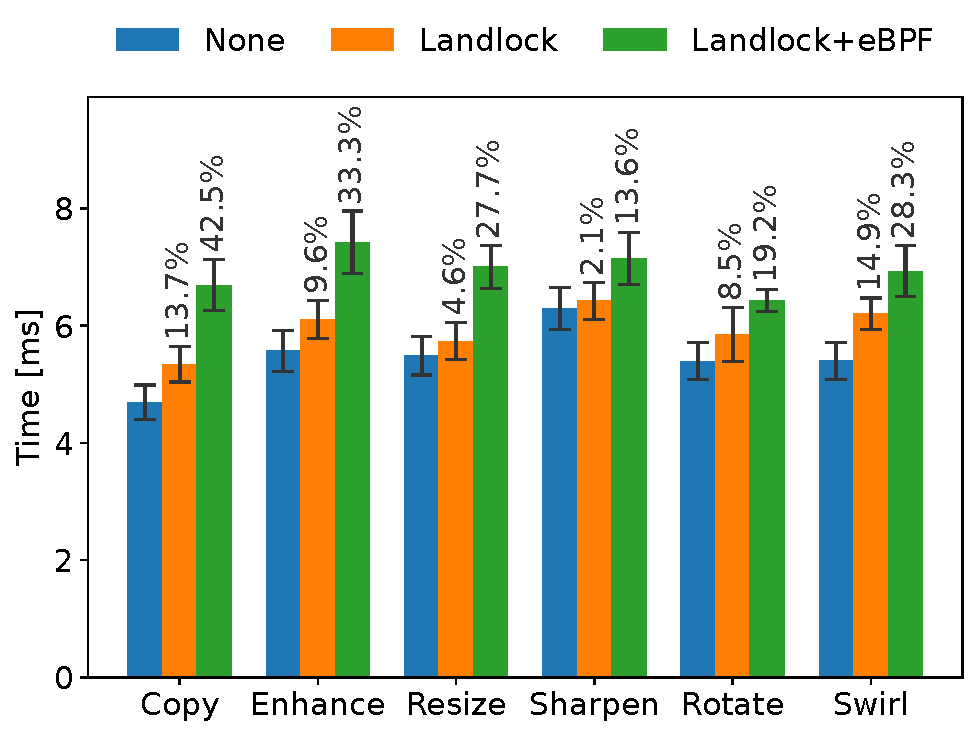
\includegraphics[width=\linewidth]{chapters/dmng/fig/convert_small.pdf}
    \caption{32x32 image resolution}
    \label{fig:convert-small-times}
  \end{subfigure}
  \begin{subfigure}[b]{0.5\linewidth}
    \centering
    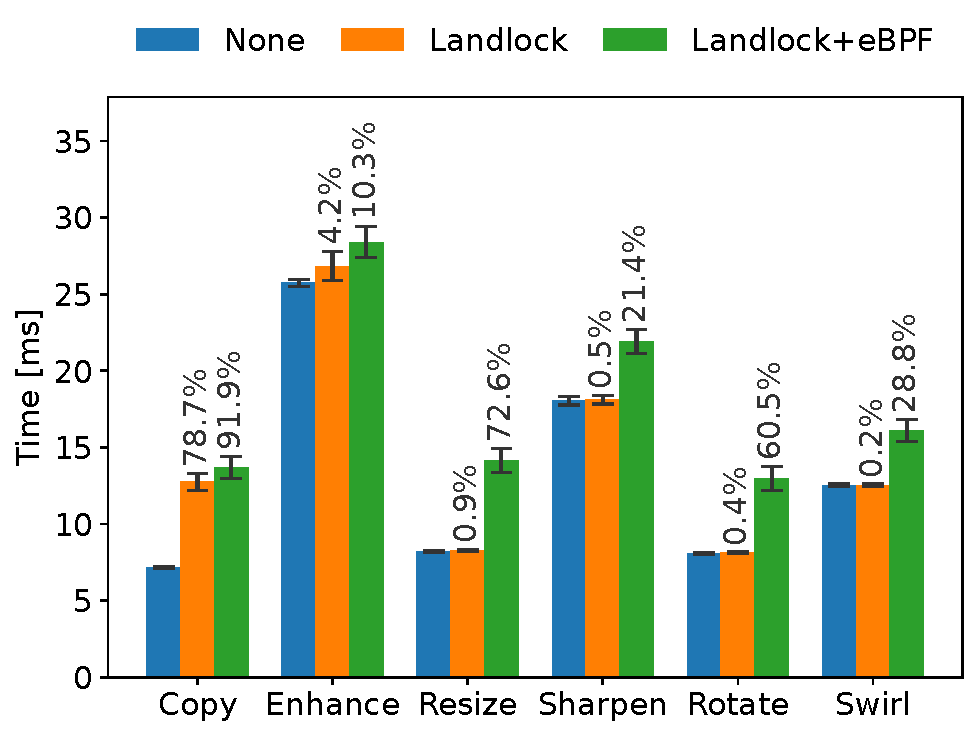
\includegraphics[width=\linewidth]{chapters/dmng/fig/convert_med.pdf}
    \caption{640x480 image resolution}
    \label{fig:convert-med-times}
  \end{subfigure}
  \begin{center}
    \begin{subfigure}[b]{0.5\linewidth}
      \centering
      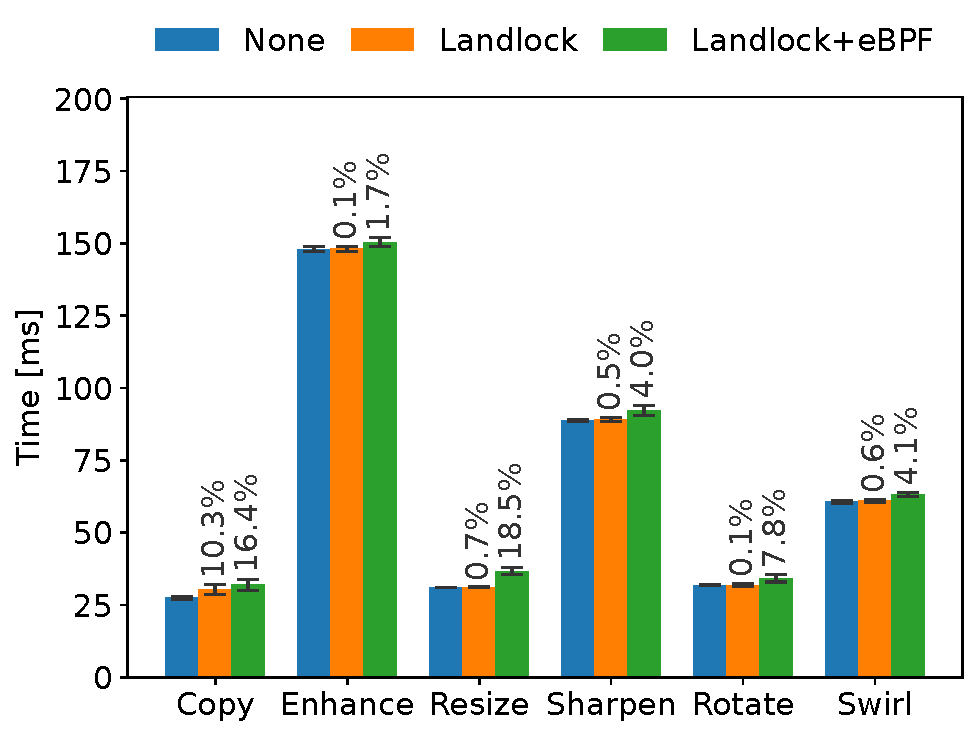
\includegraphics[width=\linewidth]{chapters/dmng/fig/convert_large.pdf}
      \caption{1920x1080 image resolution}
      \label{fig:convert-large-times}
    \end{subfigure}
  \end{center}
  \caption[Latency of image processing operations]{
      Latency associated with various operations for an image
      processing application
  }
  \label{fig:convert-times}
\end{figure*}

\begin{figure*}[t!]
  \begin{subfigure}[b]{0.5\linewidth}
    \centering
    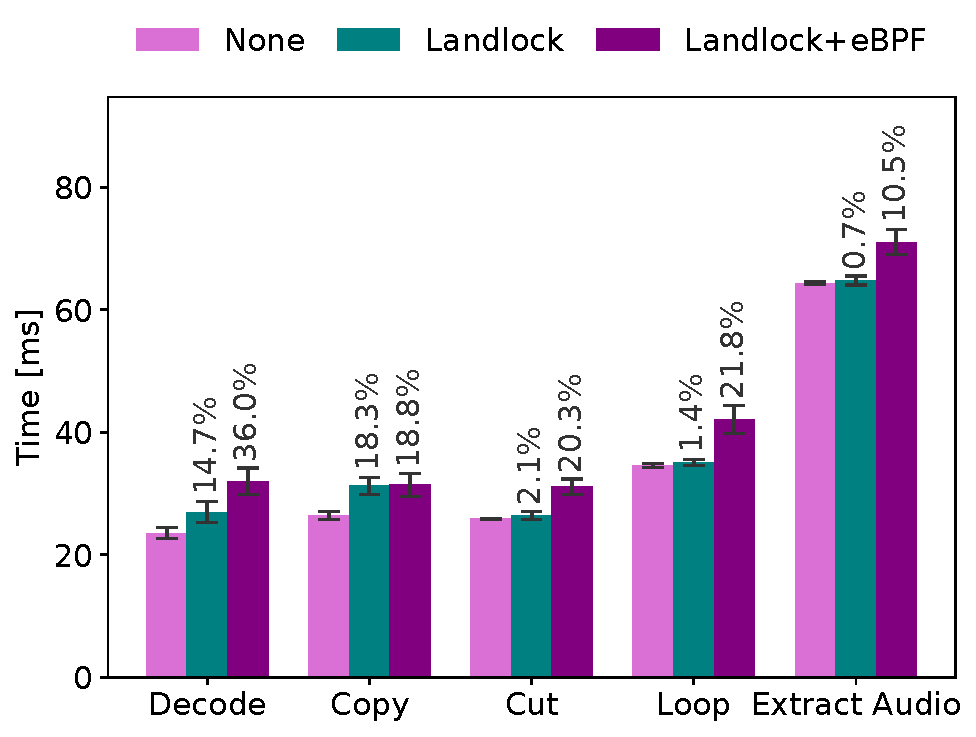
\includegraphics[width=\linewidth]{chapters/dmng/fig/ffmpeg_1.pdf}
    \caption{6 seconds 480p video}
    \label{fig:ffmpeg1-times}
  \end{subfigure}
  \begin{subfigure}[b]{0.5\linewidth}
    \centering
    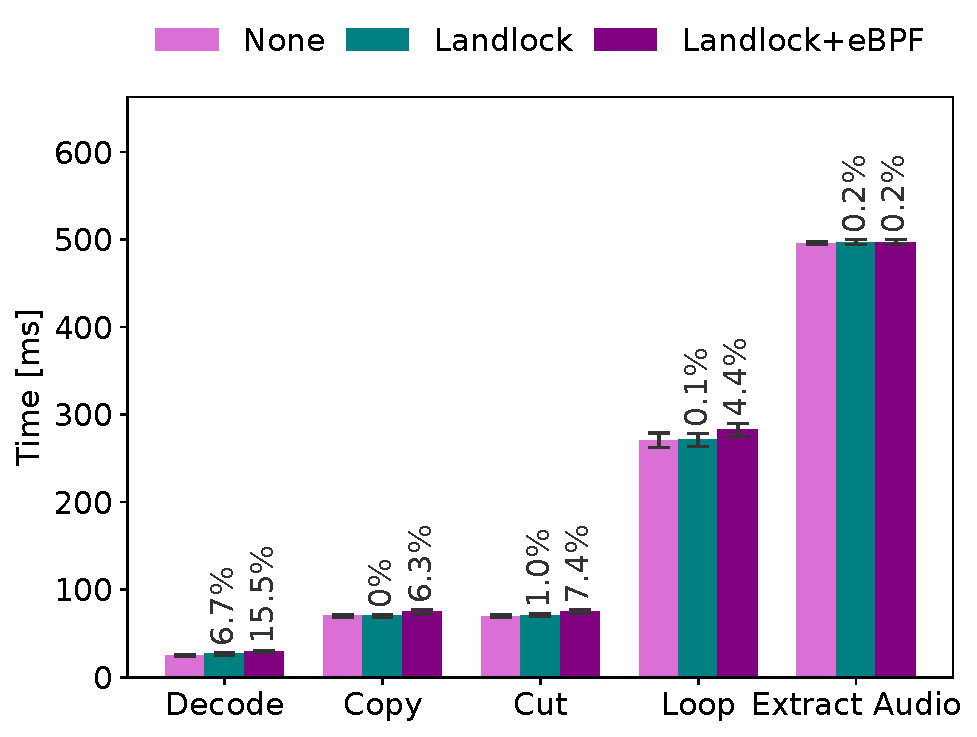
\includegraphics[width=\linewidth]{chapters/dmng/fig/ffmpeg_10.pdf}
    \caption{1 minute 480p video}
    \label{fig:ffmpeg10-times}
  \end{subfigure}
  \begin{center}
    \begin{subfigure}[b]{0.5\linewidth}
      \centering
      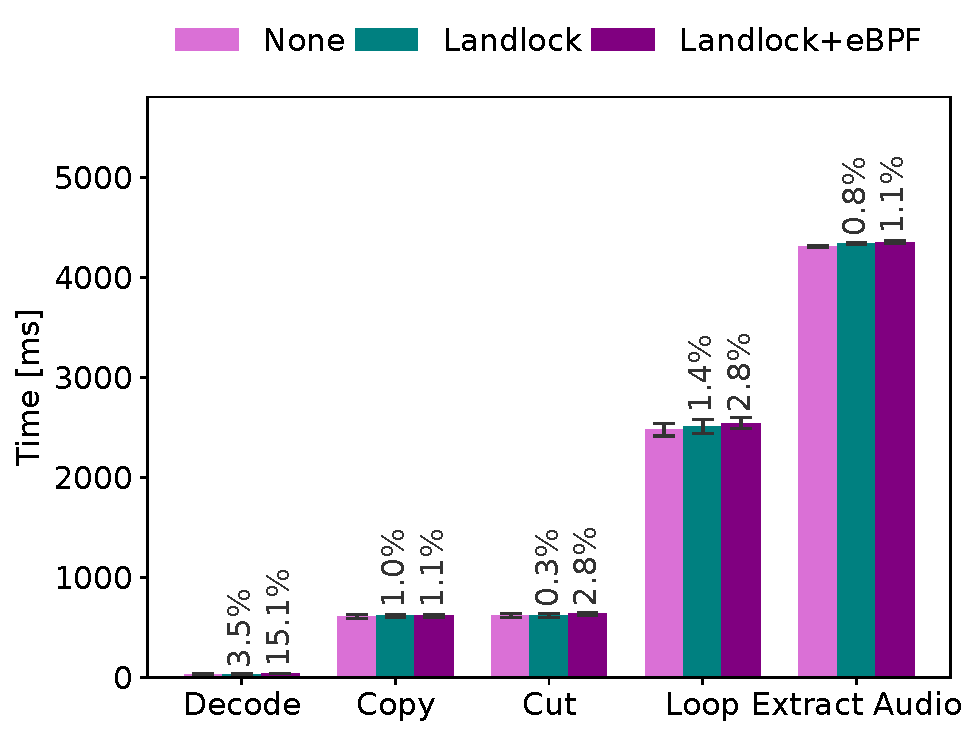
\includegraphics[width=\linewidth]{chapters/dmng/fig/ffmpeg_100.pdf}
      \caption{10 minutes 480p video}
      \label{fig:ffmpeg100-times}
    \end{subfigure}
  \end{center}
  \caption[Latency of video processing operations]{
      Latency associated with various operations for a video
      processing application
  }
  \label{fig:ffmpeg-times}
\end{figure*}

The first set of experiments focuses on image processing. In detail,
the application leverages {\em convert} to copy, enhance, resize,
sharpen, rotate and swirl images with 32x32, 640x480 and 1920x1080
resolutions. The results are shown in
Figure~\ref{fig:convert-times}. Inevitably, sandboxing introduces a
slight degradation of latency compared to a scenario without
protection.  However, the overhead is non-negligible only for
short-lived operations that last less than 10 ms, a duration that is
considerably less than the average network delay. When instead
eBPF-based monitoring is enabled, the data show worse latency
degradation, especially for operations that last less than
50~ms. Remarkable is the case 640x480, in which the average operation
overhead associated with eBPF-based monitoring is 47.6\%.

The second set of experiments focuses on video processing. In detail,
the application leverages {\em ffmpeg} to decode, copy, cut, loop and
extract audio from videos with 480p resolution and with 6 seconds, 1
minute, and 10 minutes duration respectively. The results are shown in
Figure~\ref{fig:ffmpeg-times}. The overhead introduced by sandboxing
is perceptible only for the decode and copy operations on the shortest
video (6 seconds). However, it never exceeds 18.3\%. As expected, the
overhead becomes practically negligible for operations that take
longer than 100 ms. The same considerations extend to the eBPF-based
monitoring, which again confirms to be associated with more
degradation compared to the Landlock-only solution.

%%% Local Variables:
%%% mode: latex
%%% TeX-master: "../main"
%%% End:
